\section{Архитектура и модули системы} % (fold)
\label{sec:arch_and_mod}

\subsection{Основные компоненты симулятора}
\label{sub:arch_and_mod:modules}

Для симуляции динамической оперативной памяти был выбран симулятор DRAMSim2. Данный симулятор обладает рядом преимуществ: простота, независимость от сторонних библиотек, хорошо организованная внутренняя архитектура программы. 

Симулятор является потактовым, вследствие чего все основные классы унаследованы от единого базового класса SimulatorObject. В листинге~\ref{lst:arch_and_mod:modules:simulator_object} представлена его структура. Объект этого класса имеет единственное поле - счетчик currentClockCycle, который инкрементируется методом step. Таким образом все компоненты симулятора работают в единой временной плоскости. Метод update каждый производный класс имплементирует по-своему, вкладывая нужную ему функциональность.  

\begin{lstlisting}[style=cplusplusstyle, caption={Класс SimulatorObject}, label=lst:arch_and_mod:modules:simulator_object]
class SimulatorObject
{
public:
  uint64_t currentClockCycle;

  void step();
  virtual void update()=0;
};
\end{lstlisting}

Самыми важными компонентами симулятора являются три класса: MemorySystem, MemoryController и DRAMDevice. 
Класс MemorySystem является ядром симулятора, включающим в себя всю его функциональность. Класс имеет простой интерфейс, через который внешний драйвер взаимодействует с памятью. С помощью метода AddTransaction драйвер добавляет запрос в память. Метод Update нужно вызывать в конце каждого цикла. Отсчет циклов производит драйвер памяти. 

Класс MemoryController  накапливает запросы от драйвера в очереди транзакций, транслируя их затем в команды для устройства памяти.  
Сама память представлена классом DRAMDevice, включающим в себя классы Rank и Bank. В зависимости от конфигурации каждый Rank содержит в себе определенное количество объектов Bank. В классе Bank матрица ячеек памяти представлена картой, где номер ряда является ключом, а значение представляет собой вектор слов, чьи порядковые номера соответствуют колонкам ячеек. Класс Bank представлен в листинге~\ref{lst:arch_and_mod:modules:bank}.

\begin{lstlisting}[style=cplusplusstyle, caption={Класс Bank}, label=lst:arch_and_mod:modules:bank]
class Bank
    {
    public:
        Bank();
        ~Bank();

        void read(BusPacket *busPacket);
        void write(const BusPacket *busPacket);

    public:
        BankState currentState;

    private:
        typedef map<uint64_t, std::auto_ptr<std::vector<uint16_t>> > row_map;
        row_map rowEntries;
    };
\end{lstlisting}

Для данного симулятора в открытом доступе имеется версия с возможностью хранения данных, что значительно ускорило разработку программного средства. Симулируемая память является слово-ориентированной. По этой причине появилась необходимость добавления функциональности для записи конкретных бит, а не только слов, в ячейки памяти. В листинге~\ref{lst:arch_and_mod:modules:write_bit}. представлен метод writeBit, который записывает 0 или 1 (в зависимости от параметра set) в позицию bit в ячейке по адресу заданного ряда и колонки.

\begin{lstlisting}[style=cplusplusstyle, caption={Метод записи конкретных бит в слове}, label=lst:arch_and_mod:modules:write_bit]
void Bank::writeBit(int row, int col, int bit, bool set)
{
    auto row_ = rowEntries[row].get();

    if (set)
        (*row_)[col] |= 1 << bit;
    else
    {
        if ((*row_)[col] & (1 << bit))
            (*row_)[col] ^= 1 << bit;
    }
}
\end{lstlisting}

В целом работа всей системы представляет собой следующее: контроллер памяти накапливает в очереди транзакций запросы от драйвера; на каждом новом цикле работы системы контроллер памяти извлекает одну транзакцию из очереди, транслирует её адрес в значения номера ранка, банка, ряда и колонки ячейки памяти, преобразует пакет транзакции в команду для устройства памяти и помещает этот пакет в очередь команд; из очереди команд по одному пакету в цикл извлекается команда и контроллер памяти определяет, какое действие нужно совершить устройству памяти. Решение  зависит от множества факторов: состояния банков (например, команда чтения не может быть выполнена, если адресуемая ячейка не активна, в этом случае нужна предварительная команда Activate); контроллер регенерации, который может приостановить все транзакции в системе и запустить процесс обновления памяти. Каждую команду записи в память отслеживает адаптивный сигнатурный анализатор, о котором будет рассказано в следующих подразделах. Контроллер регенерации с помощью сигнатурного анализатора выясняет, были ли неполадки в памяти за время её работы, и при необходимости запускает тесты. Внутри самого ОЗУ находится контроллер неисправностей, который имитирует поведение ячеек с физическими неисправностями, а также контролирует процесс разрядки ячеек при длительном отсутствии команды Refresh. ОЗУ в свою очередь в ответ на команды чтения возвращает контроллеру памяти считанные данные, которые сохраняются в очереди пакетов чтения и затем отправляются драйверу. Основные модули системы представлены на рисунке~\ref{fig:arch_and_mod:modules:main_modules}.

\begin{figure}[ht]
\centering
  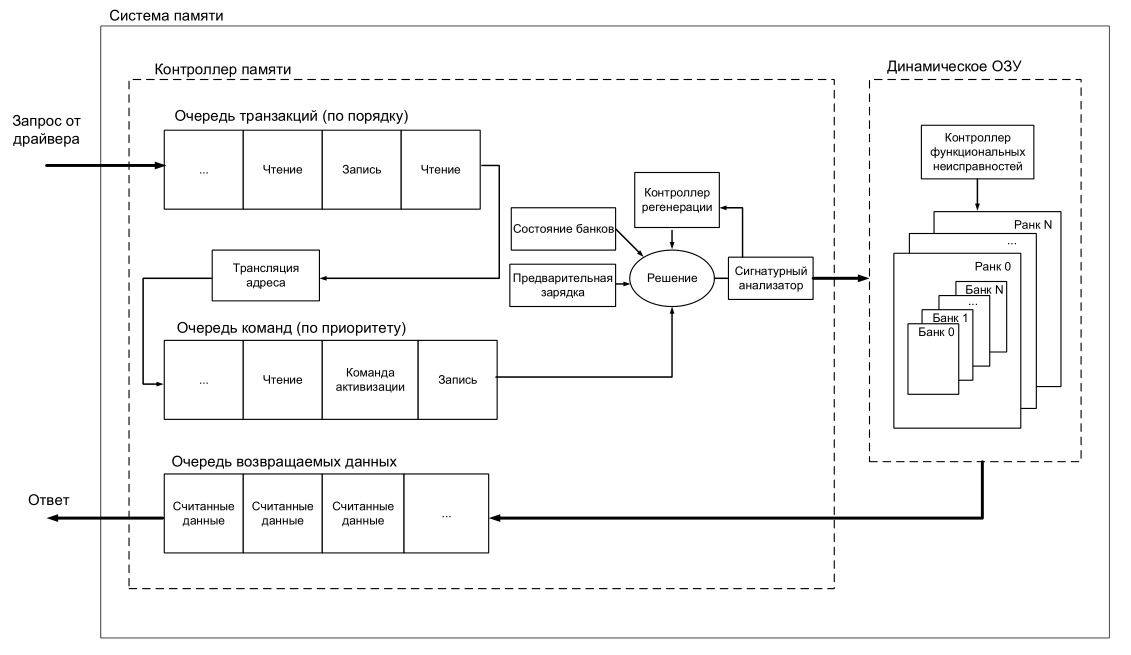
\includegraphics[scale=0.55]{a_main_modules.png}  
  \caption{ Основные компоненты симулятора ОЗУ. }
  \label{fig:arch_and_mod:modules:main_modules}
\end{figure}

\subsection{Симуляция процесса деградации памяти}
\label{sub:arch_and_mod:memory_discharge}

Источником ошибок может является свойство конденсаторов памяти разряжаться. Это происходит в случаях, когда период обновления памяти сдвинут и ячейки успевают терять свой заряд.

Этот процесс симулирует класс Discharger, который следит за периодами обновления памяти, и если такой период не наступил вовремя, то начинается постепенная деградация отдельных бит памяти в случайных местах (биты теряют свои данные и хранят 0). 

Для генерации случайных адресов ячеек и позиций бит в них используется класс uniform\_int\_distribution стандартной библиотеки шаблонов языка C++. 
Он генерирует случайные числа в диапазоне [a,b], подчинённые дискретному равномерному распределению, которое представлено на формуле~\ref{eq:arch_and_mod:memory_discharge:uniform_func} следующей функцией распределения:

\begin{equation}
  \label{eq:arch_and_mod:memory_discharge:uniform_func}
  P(i|a,b) = \frac{1}
           {b-a+1}, a \le i \ge b
\end{equation}

Плотность распределения показана на рисунке~\ref{fig:arch_and_mod:modules:uniform_distribution}.

\begin{figure}[ht]
\centering
  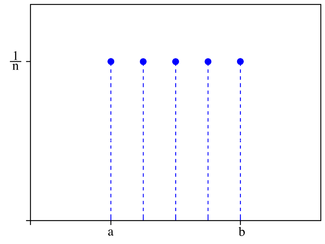
\includegraphics[scale=1]{a_uniform_distribution.png}  
  \caption{ Плотность распределения дискретного равномерного распределения. }
  \label{fig:arch_and_mod:modules:uniform_distribution}
\end{figure}

В зависимости от того, сколько циклов прошло с момента, когда должен был начаться процесс обновления памяти, количество генерируемых адресов, а следовательно количество бит, обращающихся в 0, возрастает по формуле:

\begin{equation}
  \label{eq:arch_and_mod:memory_discharge:e_func}
  f(t) = e^{\frac{\sqrt{t}}
           {5.2}}
\end{equation}

По умолчанию период обновления памяти $T_{refresh}$ = 2600 циклов. 1 цикл равен 3 нсек. Таким образом каждые 7800 нсек память должна обновляться. В итоге в соответствии с формулой примерно через 2000 циклов(с учетом погрешности генератора адресов, т.к. один и тот же адрес может сгенерироваться несколько раз) все ячейки обернутся в 0, если соответствующий процесс регенерации памяти так и не был запущен. График функции представлен на рисунке ~\ref{fig:arch_and_mod:memory_discharge:efunc_grafic}.

\begin{figure}[ht]
\centering
  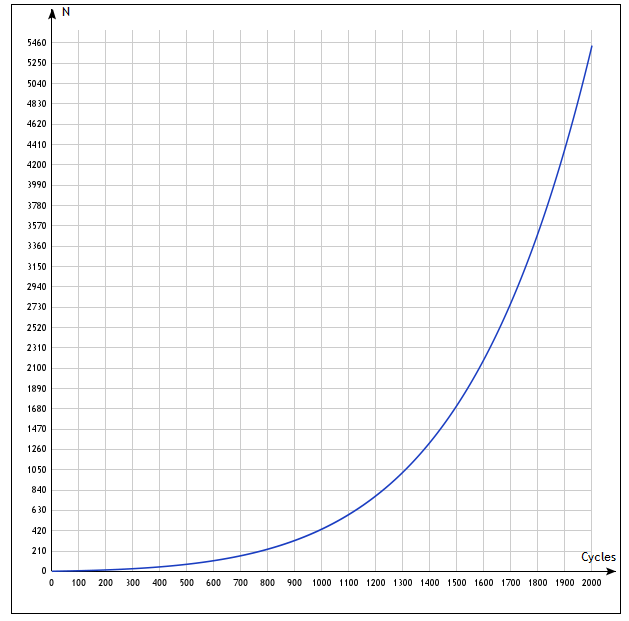
\includegraphics[scale=0.75]{a_efunc.png}  
  \caption{ График экспоненциальной функции ~\ref{eq:arch_and_mod:memory_discharge:e_func} }
  \label{fig:arch_and_mod:memory_discharge:efunc_grafic}
\end{figure}

\subsection{Симуляция процесса регенерации памяти}
\label{sub:arch_and_mod:memory_refresh}

Заряд конденсатора динамического ОЗУ со временем уменьшается вследствие утечки, поэтому для сохранения содержимого памяти процесс регенерации каждой ячейки памяти должен производится через определенное время. На время регенерации взаимодействие ОЗУ с внешними устройствами(драйвером) должно быть приостановлено, т.е. путем перевода этих устройств в режим ожидания.

В первую очередь необходимо выяснить, произошли ли ошибки во время работы памяти. Наиболее экономичным по временным затратам и эффективным методом является алгоритм адаптивного сжатия выходных данных (АСВД) (Self-Adjusting Output Data Compression - SAODC). Подробно данная технология рассмотрена в работах \cite{SAODC_Ivaniuk} и ~\cite{SAODC_Yarmolik}. Данный подход позволяет полностью избежать временных издержек для вычисления эталонной сигнатуры. Согласно этой концепции эталонная характеристика (сигнатура) $S_{ref}$ начального содержимого бит-ориентированного ОЗУ вычисляется как сумма по модулю два всех адресов ячеек, содержащих значение 1. Пример вычисления $S_{ref}$ для ОЗУ с 8 ячейками представлен на рисунке~\ref{fig:arch_and_mod:memory_refresh:saodc}.

\begin{figure}[ht]
\centering
  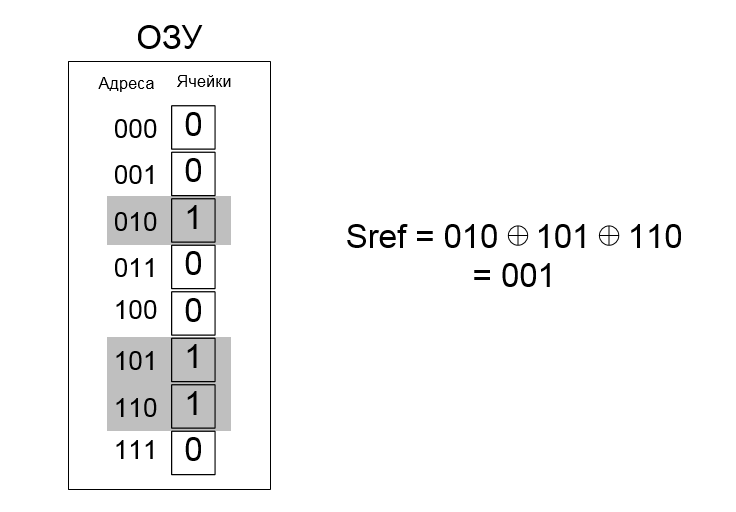
\includegraphics[scale=0.75]{a_saodc.png}  
  \caption{ Вычисление эталонной сигнатуры для бит-ориентированного ОЗУ.}
  \label{fig:arch_and_mod:memory_refresh:saodc}
\end{figure}

При таком методе изменения в памяти не потребуют заново вычислять эталонную сигнатуру, достаточно просто сложить по модулю два адрес изменившейся ячейки со значением эталонной сигнатуры. Обновление сигнатуры выглядит следующим образом:

\begin{equation}
  \label{eq:arch_and_mod:memory_refresh:adjusting_signature}
  S_{ref}^{new} = S_{ref}^{old} \oplus a \cdot ( M[a]^{new} \oplus M[a]^{old} ) \text{\,,}
\end{equation}
\begin{explanation}
где & $ a $ & адрес изменившейся ячейки; \\
    & $ M[a]^{new} $ & новое значение ячейки; \\
    & $ M[a]^{old} $ & старое значение ячейки.
\end{explanation}

Для слово-ориентированного ОЗУ применяется та же схема сжатия данных, но потребуются некоторые дополнительные действия. Пусть имеется память с матрицей ячеек 16 на 16. Т.е. 16 рядов и 16 колонок. Каждая ячейка имеет объём 8 бит. Применяя метод АСА (адаптивный сигнатурный анализатор), теперь нужно оперировать адресами не ячеек, а бит памяти. Таким образом для 5-го бита в ячейке, расположенной на 4-ом ряду и 2-ой колонке адрес будет представлен числом  0x215 в шестнадцатиричной системе счисления, или числом 0100 0010 101 в двоичной. Построение адреса бита пояснено на рисунке ~\ref{fig:arch_and_mod:memory_refresh:address}.

\begin{figure}[ht]
\centering
  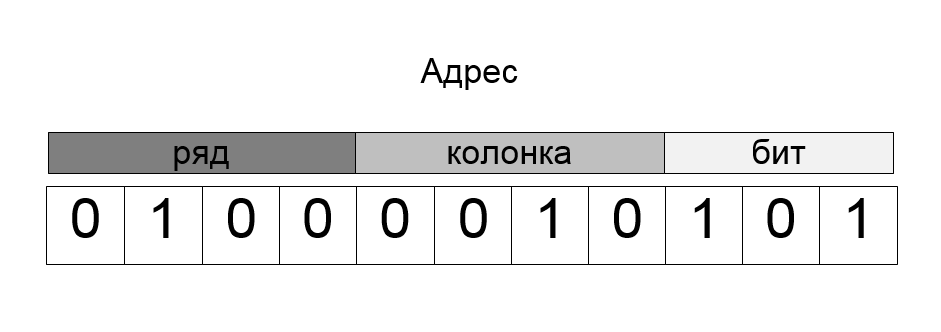
\includegraphics[scale=0.4]{a_address.png}  
  \caption{ Представление адреса бита в слово-ориентированном ОЗУ.}
  \label{fig:arch_and_mod:memory_refresh:address}
\end{figure}

У метода АСА есть недостаток, который заключается в том, что 0-вой адрес ячейки никак не повлияет на общую сумму адресов, т.к. $0 \oplus S = S$. Исходя из этого вместе с данным методом используется также бит четности\cite{March_Tests_Ivaniuk}. Бит четности - это дополнительный бит в младшем разряде адреса ячейки, который всегда содержит 1-цу. Таким образом даже нулевой адрес ячейки повлияет на общую сумму адресов. Но главная особенность бита четности заключается в том, что с его помощью можно определить, какой кратности произошла ошибка. Если тестовая и эталонная сигнатуры не совпали и бит четности равен нулю, тогда произошло четное количество ошибок, в противном случае нечетное.

После каждой операции записи в память, эталонная сигнатура обновляется. При наступлении периода регенерации, высчитывается тестовая сигнатура $S_{test}$ и затем сравнивается с эталонной $S_{ref}$. Если сигнатуры совпали - значит с памятью всё в порядке, в противном случае произошли ошибки. При однократной ошибке достаточно просто найти ядрес ячейки и позицию бита, в котором произошла ошибка. Сложение двух сигнатур  $S_{test} \oplus S_{ref}$ дает адрес бита с изменившимися данными. Таким образом процедура регенерации памяти состоит из следующих шагов:
\begin{enumerate}
  \item При наступлении периода обновления памяти вычисляется тестовая сигнатура и сравнивается с эталонной;
  \item Если сигнатуры не совпали и бит четности равен 1-це, то предполагаем, что произошла однократная ошибка. Инвертируется бит по адресу $S_{test} \oplus S_{ref}$.;
  \item Если сигнатуры не совпали и бит четности равен 0-лю, то произошло четное количество ошибок. Переход к шагу д
  \item Если сигнатуры совпали, то была однократная ошибка, которую удалось устранить. В противном случае переход к шагу д;
  \item Запуск неразрушающего маршевого теста для выявления неисправностей;
  \item Если тест ничего не обнаружил, значит была многократная ошибка, в противном случае неисправность, которую нужно диагностировать;
  \item Повторяется шаг а.
\end{enumerate}

Блок-схема алгоритма регенерации памяти представлена на рисунке ~\ref{fig:arch_and_mod:memory_refresh:refresh_chart}.

\begin{figure}[ht]
\centering
  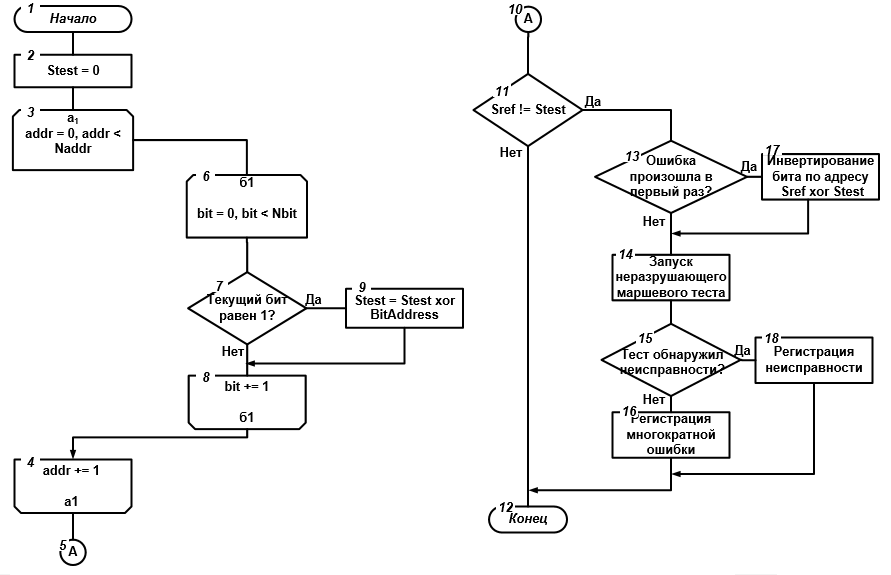
\includegraphics[scale=0.70]{a_refresh_chart.png}  
  \caption{ Схема алгоритма регенерации памяти ОЗУ.}
  \label{fig:arch_and_mod:memory_refresh:refresh_chart}
\end{figure}

За регенерацию памяти отвечает класс RegenerationController. Класс SAODCController обеспечивает вычисление рабочей и эталонной сигнатур. Метод обновления эталонной сигнатуры при каждой операции чтения представлен в листинге ~\ref{lst:arch_and_mod:memory_refresh:update_sig}

\begin{lstlisting}[style=cplusplusstyle, caption={Обновление эталонной сигнатуры ОЗУ}, label=lst:arch_and_mod:memory_refresh:update_sig]
void SAODCController::UpdateRef(BusPacket* packet)
{
    if (packet->busPacketType == DATA)
    {
        uint16_t oldData = dramDevice->read(packet->address);
        uint16_t newData = packet->data->getData();
        if (oldData != newData)
        {
            int address = GetAddress(packet->address, data);
            RefSignature ^= address;       
        }
    }
}

int SAODCController::GetAddress(int rank, int bank, int row, int col, uint16_t data)
{
    //get 'bit address sum'
    if (!data) return 0;
    
    int bitSum = 0;
    int bitCount  = 0; // '1' bit count
    for (int i = 0; (unsigned)i < DEVICE_WIDTH; i++)
    {
        if (data & (1 << i))
        {
            bitSum ^= i;
            bitCount++;
        }
    }
    if (bitCount % 2 == 0)
    addr.Clear();
    
    addr.bit = bitSum;
    int address = addr.GetPhysical();

    if (bitCount % 2 != 0)
        AddParityBit(address);
  
    return address;
}
\end{lstlisting} 

\subsection{Представление маршевых тестов}
\label{sub:arch_and_mod:march_tests}

Для выявления неисправностей ОЗУ решено использовать маршевые тесты из-за их простоты и эффективности. Все маршевые тесты построены по единому принципу и различаются лишь набором элементов. Поэтому целесообразно представить такие тесты с помощью обобщенной структуры, которая может подстроиться под любой тест. Направление перебора адресов отражается элементами MD\_UP, MD\_DOWN и MD\_BOTH перечисления MarchDirection. Операции чтения и записи также представлены элементами перечисления MarchOperation. Элементы MO\_RD и MO\_RDC обозначают операцию чтения прямого и обратного значения в буфер из ячейки памяти, элементы MO\_WD и MO\_WDC описывают операции записи прямого и обратного значения из буфера в ячейку памяти. Фаза маршевого теста отражена в структуре MarchPhase, представленной в листинге ~\ref{lst:arch_and_mod:march_tests:march_phase}.

\begin{lstlisting}[style=cplusplusstyle, caption={Структура фазы маршевого теста}, label=lst:arch_and_mod:march_tests:march_phase]
struct MarchPhase
{
    MarchDirection direction;
    std::vector<MarchOperation> elements;
};
\end{lstlisting} 

Таким образом маршевый тест представляется вектором, содержащим определённое количество структур MarchPhase. Инициализация вектора элементов маршевого теста March C- представлена в листинге ~\ref{lst:arch_and_mod:march_tests:march_init}.

\begin{lstlisting}[style=cplusplusstyle, caption={Инициализация вектора элементов маршевого теста March C-}, label=lst:arch_and_mod:march_tests:march_init]
void InitializeTest()
{
    std::vector<MarchPhase> phases;
    phases.push_back({ MD_UP, { MO_RD, MO_WDC } });
    phases.push_back({ MD_UP, { MO_RDC, MO_WD } });
    phases.push_back({ MD_DOWN, { MO_RD, MO_WDC } });
    phases.push_back({ MD_DOWN, { MO_RDC, MO_WD } });
    phases.push_back({ MD_DOWN, { MO_RD } });
};
\end{lstlisting} 

Другие виды маршевых тестов инициализируются подобным образом. Программа поддерживает следующие маршевые тесты: March C-, March A, March B, March X, March Y, MATS, MATS+, MATS++.

Логика создания и выполнения маршевых тестов находится в классе MarchTestController. Запуск теста производит класс RegenerationController. Для сжатия данных используется адаптивный сигнатурный анализатор, рассмотренный в предыдущем пункте. На этапе инициализации теста в качестве эталонной сигнатуры берётся уже вычисленная ранее рабочая сигнатура класса RegenerationController. Далее на каждой фазе маршевого теста вычисляется тестовая сигнатура и в конце фазы сравнивается с эталонной. При правильном функционировании памяти сигнатуры должны всегда совпадать вне зависимости от операций, производимых элементами маршевого теста. Это происходит потому, что маршевый тест является неразрушающим, а также благодаря свойству АСА, которое заключается в равенстве сумм адресов ячеек, содержащих 1, и адресов ячеек, содержащих 0. Выполнение маршевого теста занимает определённое время, а потому выполнение отдельных его фаз разбито на несколько циклов работы симулятора. Выполнение теста приводится в листинге ~\ref{lst:arch_and_mod:march_tests:march_run}.

\begin{lstlisting}[style=cplusplusstyle, caption={Функция выполнения маршевого теста}, label=lst:arch_and_mod:march_tests:march_run]
void MarchTestController::Update()
{
    if (!state.testStarted) return;

    saodc.ClearTestSig();
    MarchPhase& phase = phases[state.phase];
    int addrStart = 0;
    int counter = 0;
    int bottom = 0;
    int top = NUM_BANKS * NUM_COLS * NUM_ROWS - 1;

    if (phase.direction == MD_UP || phase.direction == MD_BOTH)
    {
        addrStart = bottom;
        counter = 1;
    }
    else if (phase.direction == MD_DOWN)
    {
        addrStart = top;
        counter = -1;
    }
    for (int addr = addrStart; addr >= bottom && addr <= top; addr += counter)
    {
        uint16_t buffer = 0;
        uint16_t old = 0;
        for (auto& el : phase.elements)
        {
            RunElement(el, addr, buffer, old);
        }
    }
    int err = saodc.Compare();
    if (err)
    {
        state.testPassed = false;
        cout << "[MarchTest] Errors are detected while running phase! Signature sum is " << err << "(" << addrTranslator.GetDescription(err, true) << ")" << endl;
    }
    state.phase++;
    if (state.phase == phases.size())
    {
        state.testCompleted = true;
        state.testStarted = false;
    }
}
\end{lstlisting} 

Выполнение каждой отдельной операции маршевого элемента приведено в листинге ~\ref{lst:arch_and_mod:march_tests:march_element_run}.

\begin{lstlisting}[style=cplusplusstyle, caption={Выполнение элемента маршевого теста}, label=lst:arch_and_mod:march_tests:march_element_run]
void MarchTestController::RunElement(int element, int address, uint16_t &buffer, uint16_t& oldValue)
{
    int r = 0, b = 0, row = 0, col = 0;
    addrTranslator.Translate(address, r, b, row, col);
    uint16_t data = 0;
    switch (element)
    {
    case MO_RD:
        data = dramDevice->read(r, b, row, col);
        buffer = data;
        break;
    case MO_RDC:
        data = dramDevice->read(r, b, row, col);
        buffer = ~data;
        break;
    case MO_WD:
        dramDevice->write(r, b, row, col, buffer);
        break;
    case MO_WDC:
        dramDevice->write(r, b, row, col, ~buffer);
        break;
    }
    //convertData
    if (element == MO_RD || element == MO_RDC)
    {
        saodc.UpdateTestSig(addr, data ^ oldValue);
        oldValue = data;
    }
}
\end{lstlisting} 

\subsection{Моделирование функциональных неисправностей ОЗУ}
\label{sub:arch_and_mod:faults}

Для моделирования функциональных неисправностей ОЗУ используется обобщенная структура Fault, представленная в листинге~\ref{lst:arch_and_mod:faults:faults_struct}. 
\begin{lstlisting}[style=cplusplusstyle, caption={Структура описания функциональной неисправности ОЗУ}, label=lst:arch_and_mod:faults:faults_struct]
struct Fault
{
    FaultType type;
    uint16_t victimVal;
    uint16_t agressorVal;
    int agressorAddr;
};
\end{lstlisting} 

Поле type может принимать одно из следующих значений: SAF,TF, AF, CFin, CFid, CFst. Они объединены в перечислении FaultType. Поле victimVal для разных моделей неисправностей имеет различное значение, но обобщенно оно хранит значение ячейки-жертвы. Так для неисправностей типа SAF victimVal будет содержать значение ячейки памяти, которое эта ячейка хранит постоянно и изменить его не может. Для неисправности TF это поле хранит значение, перейдя в которое ячейка превращается в константную, т.е. не может поменять своё состояние. Для неисправностей CFid и CFst данное поле хранит значение, в которое зависимая ячейка принудительно переходит (для CFid) или в которое она может перейти только при определённом значении в ячейке-агрессоре (для CFst). Для неисправностей типа CFin и AF данное поле не неиспользуется. 

Поле agressorAddr хранит адрес ячейки-агрессора. Это поле используется в неисправностях типа CF и AF. Поле agressorVal используется только для CF. Поле agressorVal хранит значение ячейки-агрессора, при котором зависимая ячейка может перейти в состояние victimVal (для CFst) или значение, при переходе в которое, ячейка-жертва насильно меняет своё значение на victimVal (для CFin и CFid). Для неисправности типа AF поле agressorAddr хранит адрес ячейки, при записи значения в которую записываемое значение дублируется по адресу ячейки-жертвы.

Класс, контролирующий поведение ячеек в соответствии с различными моделями неисправностей, называется FaultController и находится в классе DRAMDevice. При каждой операции записи в память FaultController вмешивается в работу системы и имитирует поведение неисправностей. Все основные виды неисправностей выявляются на протяжении работы симулятора, однако при неисправностях типа SAF необходимо инициализировать значения ячеек памяти на старте симулятора. 

Метод, анализирующий операцию записи в ячейку памяти и принимающий решение о выполнении тех или иных действий, соответствующих моделям неисправностей, представлен в листинге~\ref{lst:arch_and_mod:faults:faults_run}.

\begin{lstlisting}[style=cplusplusstyle, caption={Реализаия поведения ячеек с функциональными неисправностями}, label=lst:arch_and_mod:faults:faults_run]
void FaultController::DoFaults(Address addr, uint16_t data)
{
    uint16_t oldData = dramDevice->read(addr);
    uint16_t bitMask = oldData ^ data;
  
    for (unsigned i = 0; i < DEVICE_WIDTH; i++)
    {
        if (bitMask & (1 << i))
        {
            addr.bit = i;
            DoOperationOnBit(addr, data & (1 << i) ? 1 : 0, oldData & (1 << i) ? 1 : 0);
        }
    }
}

void FaultController::DoOperationOnBit(Address address, uint16_t newVal, uint16_t oldVal)
{
    int addr = address.GetPhysical();
    if (IsFaulty(addr))
    {
        Fault fault = GetCellAttributes(addr, false);
        switch (fault.type)
        {
            case SAF: break;
            case TF:
            {
                if (oldVal != fault.victimValue)
                {
                    WriteBit(address, newVal);
                }
                break;
            }
            case CFin:
            {
                WriteBit(address, newVal);
                break;
            }     
            case CFid:
            {
                WriteBit(address, newVal);
                break;
            }
            case CFst:
            {
                if (newVal != fault.victimValue)
                    WriteBit(address, newVal);
                else
                {
                    Address agrAdr(fault.agressorAddress, true);
                    if (dramDevice->readBit(agrAdr) == fault.agressorValue)
                        WriteBit(address, newVal);
                }
                break;
            }
            default: break;
        }
    }
    else
    {
        if (IsAgressor(addr))
        {
            Fault fault = GetCellAttributes(addr, true);      
            switch (fault.type)
            {
                case CFin:
                {
                    if (newVal == fault.agressorValue && newVal != oldVal)
                    {
                        Address vicAdr(fault.victimAddress, true);
                        (*dramDevice->ranks)[vicAdr.rank].banks[vicAdr.bank].invertBit(vicAdr);
                    }
                    break;
                }
                case CFid:
                {
                    if (newVal == fault.agressorValue && newVal != oldVal)
                    {
                        Address vicAdr(fault.victimAddress, true);
                        WriteBit(vicAdr, fault.victimValue);
                    }
                    break;
                }
                case AF:
                {
                    Address vicAdr(fault.victimAddress, true);
                    WriteBit(vicAdr, newVal);
                    break;
                }
                default :
                  break;
            }
            WriteBit(address, newVal);
        }
        else
        {
            WriteBit(address, newVal);
        }
    } 
}
\end{lstlisting} 


\subsection{Верификация неразрушающих маршевых тестов}
\label{sub:arch_and_mod:verification}

Для верификации были взяты следующие неразрушающие маршевые тесты: March C-, March A, March B, March X, March Y, MATS, MATS+, MATS++. Описание тестов находится в таблице \ref{table:arch_and_mod:verification:march_tests}.


\begin{table}[ht]
  \caption{Неразрушающие маршевые тесты}
  \label{table:arch_and_mod:verification:march_tests}
  \begin{tabular}{| >{\centering}m{0.15\textwidth}
                  | >{\centering}m{0.15\textwidth}
                  | >{\centering\arraybackslash}m{0.6\textwidth}|}
   \hline 
  {Название} & {Сложность} & {Описание теста} \\ \hline
   March C- & 9N & $\{\Uparrow (rd,wdc); \Uparrow (rdc,wd); \Downarrow (rd,wdc); \Downarrow (rdc,wd); \Updownarrow (rd)\}$ \\ \hline
   March A & 14N & $\{\Uparrow(rd,wdc,wd,wdc); \Uparrow (rdc,wd,wdc); \Downarrow (rdc,wd,wdc,wd); \Downarrow (rd,wdc,wd)\}$ \\ \hline
   March B & 16N & $\{\Uparrow(rd,wdc,rdc,wd,rd,wdc); \Uparrow (rdc,wd,wdc); \Downarrow (rdc,wd,wdc,wd); \Downarrow (rd,wdc,wd)\}$ \\ \hline
   March X & 5N & $\{\Uparrow (rd,wdc); \Downarrow (rdc,wd); \Updownarrow (rd)\}$ \\ \hline
   March Y & 5N & $\{\Uparrow (rd,wdc,rdc); \Downarrow (rdc,wd,rd); \Updownarrow (rd)\}$ \\ \hline
   MATS & 3N & $\{\Updownarrow (rd,wdc); \Updownarrow (rdc)\}$ \\ \hline
   MATS+ & 4N & $\{\Uparrow (rd,wdc); \Downarrow (rdc,wd)\}$ \\ \hline
   MATS++ & 5N & $\{\Uparrow (rd,wdc); \Downarrow (rdc,wd,rd)\}$ \\ \hline   
  \end{tabular}
\end{table}

Для верификации потребовалось запустить каждый тест для каждой модели неисправности, находящейся в памяти. Всего были проверены 26 неисправностей: 2 вида SAF, 2 вида TF, 2 вида AF, 4 вида CFin, 8 видов CFid и 8 видов CFst. В качестве неисправностей AF были взяты только два случая: когда адрес ячейки, чье значение при записи дублируется в ячейку-жерту, меньше, чем адрес ячейки-жертвы, и наоборот. 

Для неисправностей SAF, TF, AF и CFin результаты тестов приведены в таблице \ref{table:arch_and_mod:verification:coverage1}.

\begin{table}[!ht]
\caption{Покрывающая способность неразрушающих маршевых тестов неисправностей SAF, TF, AF и CFin}
\label{table:arch_and_mod:verification:coverage1}
  \centering
  \begin{tabular}{| >{\centering}m{0.13\textwidth} 
                  | >{\centering}m{0.02\textwidth} 
                  | >{\centering}m{0.02\textwidth} 
                  | >{\centering}m{0.02\textwidth} 
                  | >{\centering}m{0.02\textwidth} 
                  | >{\centering}m{0.05\textwidth} 
                  | >{\centering}m{0.05\textwidth} 
                  | >{\centering}m{0.1\textwidth} 
                  | >{\centering}m{0.1\textwidth} 
                  | >{\centering}m{0.1\textwidth} 
                  | >{\centering\arraybackslash}m{0.1\textwidth}|}
    \hline
    \multirow{3}{0.13\textwidth}{\centering Тест} & \multicolumn{10}{c|}{Модели неисправностей} \\ \cline{2-11}    
    & \multicolumn{2}{c|}{SAF} & \multicolumn{2}{c|}{TF} & \multicolumn{2}{c|}{AF} & \multicolumn{4}{c|}{CFin} \\ \cline{2-11}
    & 0 & 1 & $\downarrow$ & $\uparrow$ & $\wedge(b)$ & $\vee(b)$ & $\wedge(\uparrow,b)$ & $\wedge(\downarrow,b)$ & $\vee(\uparrow,b)$ & $\vee(\downarrow,b)$ \\ \hline
    
    March C-  & + & + & + & + & + & + & + & + & + & +\\ \hline
    March A   & + & + & + & + & + & + & + & + & + & +\\ \hline
    March B   & + & + & + & + & + & + & + & + & + & +\\ \hline
    March X   & + & + & + & + & + & + & + & + & + & +\\ \hline
    March Y   & + & + & + & + & + & + & + & + & + & +\\ \hline
    MATS      & + & + & + & - & + & - & + & - & + & -\\ \hline
    MATS+     & + & + & + & - & + & + & + & - & + & +\\ \hline
    MATS++    & - & - & - & + & + & + & + & - & + & +\\ \hline
  \end{tabular}
\end{table}

Для неисправностей CFid результаты тестов приведены в таблице \ref{table:arch_and_mod:verification:coverage2}.

\begin{table}[!ht]
\caption{Покрывающая способность неразрушающих маршевых тестов неисправностей CFid}
\label{table:arch_and_mod:verification:coverage2}
  \centering
  \begin{tabular}{| >{\centering}m{0.12\textwidth} 
                  | >{\centering}m{0.075\textwidth} 
                  | >{\centering}m{0.075\textwidth} 
                  | >{\centering}m{0.075\textwidth} 
                  | >{\centering}m{0.075\textwidth} 
                  | >{\centering}m{0.075\textwidth} 
                  | >{\centering}m{0.075\textwidth} 
                  | >{\centering}m{0.075\textwidth} 
                  | >{\centering\arraybackslash}m{0.1\textwidth}|}
    \hline
    \multirow{3}{0.12\textwidth}{\centering Тест} & \multicolumn{8}{c|}{Модели неисправностей} \\ \cline{2-9}    
    & \multicolumn{8}{c|}{CFid} \\ \cline{2-9}
    & {$\wedge$ \\ $(\uparrow,0)$} & {$\wedge$ \\ $(\uparrow,1)$} & {$\wedge$ \\ $(\downarrow,0)$} & {$\wedge$ \\ $(\downarrow,1)$} 
    & {$\vee$ \\ $(\uparrow,0)$} & {$\vee$ \\ $(\uparrow,1)$} & {$\vee$ \\ $(\downarrow,0)$} & $\vee(\downarrow,1)$ \\ \hline
    
    March C-  & + & + & + & + & + & + & + & + \\ \hline
    March A   & + & + & + & + & + & + & + & + \\ \hline
    March B   & + & + & + & + & + & + & + & + \\ \hline
    March X   & - & + & - & + & + & - & + & - \\ \hline
    March Y   & - & + & - & + & + & - & + & - \\ \hline
    MATS      & - & + & - & - & + & - & - & - \\ \hline
    MATS+     & - & + & - & - & + & - & + & - \\ \hline
    MATS++    & - & + & - & - & + & - & + & - \\ \hline
  \end{tabular}
\end{table}

Для неисправностей CFst результаты тестов приведены в таблице \ref{table:arch_and_mod:verification:coverage3}.

\begin{table}[!ht]
\caption{Покрывающая способность неразрушающих маршевых тестов неисправностей CFst}
\label{table:arch_and_mod:verification:coverage3}
  \centering
  \begin{tabular}{| >{\centering}m{0.12\textwidth} 
                  | >{\centering}m{0.075\textwidth} 
                  | >{\centering}m{0.075\textwidth} 
                  | >{\centering}m{0.075\textwidth} 
                  | >{\centering}m{0.075\textwidth} 
                  | >{\centering}m{0.075\textwidth} 
                  | >{\centering}m{0.075\textwidth} 
                  | >{\centering}m{0.075\textwidth} 
                  | >{\centering\arraybackslash}m{0.1\textwidth}|}
    \hline
    \multirow{3}{0.12\textwidth}{\centering Тест} & \multicolumn{8}{c|}{Модели неисправностей} \\ \cline{2-9}    
    & \multicolumn{8}{c|}{CFst} \\ \cline{2-9}
    & {$\wedge$ \\ $(0,0)$} & {$\wedge$ \\ $(0,1)$} & {$\wedge$ \\ $(1,0)$} & {$\wedge$ \\ $(1,1)$} 
    & {$\vee$ \\ $(0,0)$} & {$\vee$ \\ $(0,1)$} & {$\vee$ \\ $(1,0)$} & $\vee(1,1)$ \\ \hline
    
    March C-  & + & + & + & + & + & + & + & + \\ \hline
    March A   & + & + & - & - & - & + & + & + \\ \hline
    March B   & + & + & - & - & - & + & + & + \\ \hline
    March X   & + & + & - & - & - & - & + & + \\ \hline
    March Y   & + & + & - & - & - & - & + & + \\ \hline
    MATS      & - & + & - & - & - & - & - & + \\ \hline
    MATS+     & - & + & - & - & - & - & - & + \\ \hline
    MATS++    & + & - & - & - & - & - & + & - \\ \hline
  \end{tabular}
\end{table}

Обобщенные результаты по всем тестам представлены в таблице\ref{table:arch_and_mod:verification:coverage}.

\begin{table}[!ht]
\caption{Покрывающая способность неразрушающих маршевых тестов}
\label{table:arch_and_mod:verification:coverage}
  \centering
  \begin{tabular}{| >{\centering}m{0.2\textwidth} 
                  | >{\centering}m{0.1\textwidth} 
                  | >{\centering}m{0.1\textwidth} 
                  | >{\centering}m{0.1\textwidth} 
                  | >{\centering}m{0.1\textwidth} 
                  | >{\centering}m{0.1\textwidth} 
                  | >{\centering\arraybackslash}m{0.1\textwidth}|}
    \hline
    \multirow{2}{0.15\textwidth}{\centering Тест} &
    \multicolumn{6}{c|}{\centering Модели неисправностей} \\
    \cline{2-7}
    & SAF & TF & AF & CFin & CFid & CFst \\
    \hline
     March C-   & 2/2 & 2/2 & 2/2 & 4/4 & 8/8 & 8/8 \\ \hline
     March A    & 2/2 & 2/2 & 2/2 & 4/4 & 8/8 & 5/8 \\ \hline
     March B    & 2/2 & 2/2 & 2/2 & 4/4 & 8/8 & 5/8 \\ \hline
     March X    & 2/2 & 2/2 & 2/2 & 4/4 & 4/8 & 4/8 \\ \hline
     March Y    & 2/2 & 2/2 & 2/2 & 4/4 & 4/8 & 4/8 \\ \hline
     MATS       & 2/2 & 1/2 & 1/2 & 2/4 & 2/8 & 2/8 \\ \hline
     MATS+      & 2/2 & 1/2 & 2/2 & 3/4 & 3/8 & 2/8 \\ \hline
     MATS++     & 0/2 & 1/2 & 2/2 & 3/4 & 3/8 & 2/8 \\ \hline
  \end{tabular}
\end{table}

Из результатов тестов видно, что наибольшей покрывающей способностью обладает маршевый тест March C-. По сравнению с тестами March A и March B, которые также имеют хорошие показатели обнаружения неисправностей, тест March C- не только охватывает больше неисправностей, но и является оптимальным по скорости по сравнению с предыдущими тестами. 





